%!TeX root=../apresentacao.tex
%("dica" para o editor de texto: este arquivo é parte de um documento maior)
% para saber mais: https://tex.stackexchange.com/q/78101/183146

% Apague as duas linhas abaixo (elas servem apenas para gerar um
% aviso no arquivo PDF quando não há nenhum dado a imprimir) e
% insira aqui o conteúdo do seu trabalho. Tome por base o
% arquivo corpo-apresentacao.tex do diretório conteudo-exemplo
% para a definição do título, autoria etc. e estrutura da
% apresentação.

\input{extras/aviso-conteudo}
\avisoApresentacao
%%%%%%%%%%%%%%%%%%%%%%%%%%%%%%%%% METADADOS %%%%%%%%%%%%%%%%%%%%%%%%%%%%%%%%%%%%

\title[Visualização de Dados do Tráfego]{Visualização de Fluxos de Mobilidade Urbana com \emph{Bundling}}
% \subtitle{The (optional) subtitle}

\author[Tallys Martins]{Tallys Martins}

%\institute[USP]{\textbf{Workshop Name} \\ Computer Science Department \\ IME USP}
\institute[USP]{
 \textbf{Orientador:} Fabio Kon \\
 Departamento de Ciência da Computação \\ IME USP
}

\date{Janeiro de 2021}

% Coloca a imagem no fundo da página de título
\bgimage{\includegraphics[width=\paperwidth]{fundo_predios_e_grafo}}

% Logotipos no rodapé da página de título
\logos{
  \hfil\hfil\includegraphics[width=.1\textwidth]{usp-logo}\hfil%
  \raisebox{-.0103\paperheight}{\includegraphics[height=.0932\paperheight]{interscity-logo}}\hfil%
  \raisebox{-.033\paperheight}{\includegraphics[width=.07\textwidth,trim=0 230 0 0,clip]{ime-logo}}\hfil\hfil
}

%\logos{
%  \hfil\hfil\includegraphics[width=.1\textwidth]{usp-logo}\hfil%
%  \raisebox{-.0103\paperheight}{\includegraphics[height=.0932\paperheight]{interscity-logo}}\hfil%
%  \raisebox{-.00517\paperheight}{\includegraphics[height=.057\paperheight]{cnpq-logo}}\hfil%
%  \raisebox{-.0342\paperheight}{\includegraphics[height=.1035\paperheight]{capes-logo}}\hfil%
%  \includegraphics[height=.044\paperheight]{fapesp-logo}\hfil\hfil
%}

% Usado para criar o qrcode com o endereço da apresentação
% \presentationurl{http://interscity.org}

% Inclui o qrcode no sumário da apresentação
% \includeqrcodeintoc

% O slide de sumário pode ser dividido em colunas; o parâmetro
% determina após qual o número da seção fazer a quebra de coluna
% (use zero para uma coluna ou simplesmente omita este comando).
\toccolumns{4}

%%%%%%%%%%%%%%%%%%%%%%%%%%%%%%%%%%%%%%%%%%%%%%%%%%%%%%%%%%%%%%%%%%%%%%%%%%%%%%%%
%%%%%%%%%%%%%%%%%%%%%%%%%%%% INÍCIO DA APRESENTAÇÃO %%%%%%%%%%%%%%%%%%%%%%%%%%%%
%%%%%%%%%%%%%%%%%%%%%%%%%%%%%%%%%%%%%%%%%%%%%%%%%%%%%%%%%%%%%%%%%%%%%%%%%%%%%%%%

% É complicado colocar uma imagem de fundo, os logos das agências e
% o conteúdo "normal" do slide de título sem que as coisas fiquem
% bagunçadas, então definimos um comando para gerar o slide de título
\customtitlepage

% Slide com o qrcode
\showqrcode

\begin{frame}{Agenda}
  \overview
\end{frame}

\section{Introdução}

% O trabalho é sobre dados do tráfego, então nada mais justo do que começar
% explicando o que é o tráfego e que estamos interessados no trânsito
% Pode ressaltar que 40% da população mundial gasta pelo menos 1h por dia no trânsito
% E também pode falar que esses dados na cidade são coletados com os avanços
% nos sistemas de transporte
\begin{frame}{Dados de Tráfego}
  ``Tráfego em uma via é o fluxo ou a passagem de veículos e pedestres por um
caminho que pode ser em regiões urbanas, mares, no ar e até no subsolo''

\hfill \citep{Chen2015}

  \begin{figure}[h!]
    \centering
    \begin{subfigure}{0.20\textwidth}
      \centering
      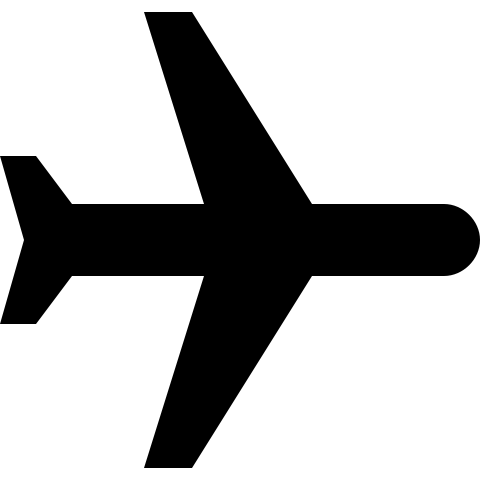
\includegraphics[width=.4\textwidth]{black-plane.png}
    \end{subfigure}
    ~
    \begin{subfigure}{0.20\textwidth}
      \centering
      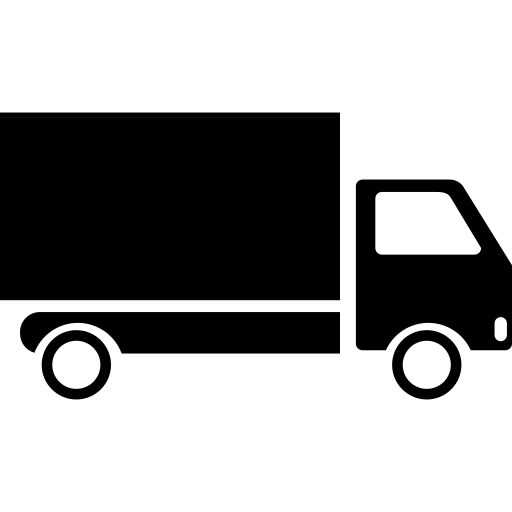
\includegraphics[width=.4\textwidth]{delivery-truck.png}
    \end{subfigure}
    ~
    \begin{subfigure}{0.20\textwidth}
      \centering
      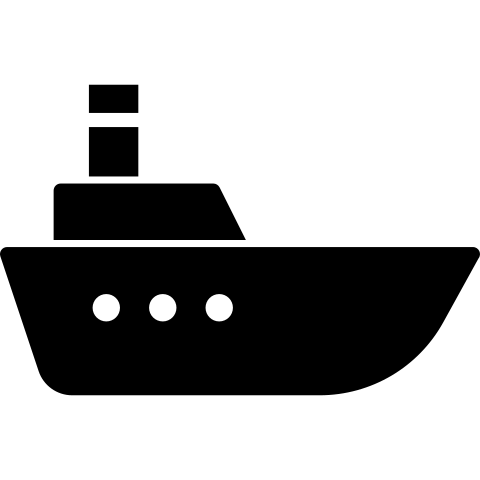
\includegraphics[width=.4\textwidth]{sea-ship.png}
    \end{subfigure}
    ~
    \begin{subfigure}{0.20\textwidth}
      \centering
      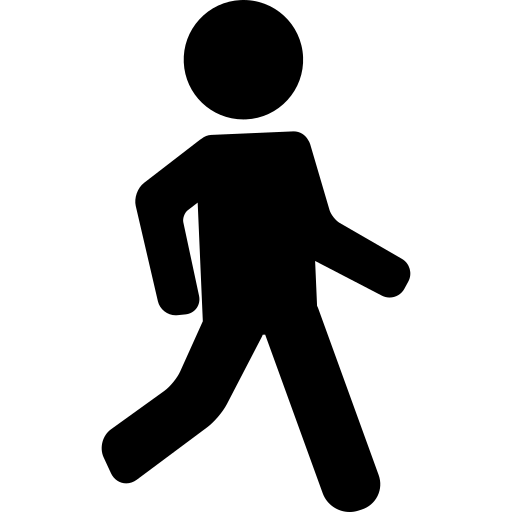
\includegraphics[width=.4\textwidth]{one-man-walking.png}
    \end{subfigure}
  \end{figure}
\end{frame}

%\begin{frame}[plain]
%  \includegraphics[width=\textwidth]{interscity-logo}
%\end{frame}

% Aqui eu falo de mais algumas características sobre os dados do tráfego e
% como eles podem auxiliar no planejamento das cidades
% o que dá uma noção da complexidade de análise desses dados
\begin{frame}{Dados de Tráfego}
  \begin{itemize}
    \item Relações de deslocamento entre regiões
    \item Multidimensionais (posição, velocidade, aceleração)
    \item Volumosos (\emph{big data})
  \end{itemize}
\end{frame}


\begin{frame}{Problemas}
  \begin{itemize}
    \item Que regiões recebem os maiores fluxos de veículos?
    \item Que regiões são responsáveis pelo maior fluxo em uma via?
    \item Como os fluxos de deslocamento se comportam ao longo do dia?
    \item Como os fluxos se comportam com eventos atípicos?
  \end{itemize}
\end{frame}

% Aqui eu falo no que estamos interessados... criar uma visualização desses fluxos
% para, por exemplo, responder as questões do próximo slide

% falar que vamos fazer isso com dados reais e simulados?
\begin{frame}[standout]
  Visualização dos fluxos de origem e destino no tráfego de veículos no
trânsito da cidade
\end{frame}


% Aqui eu falo que eles podem ser representados como um grafo e que essa representação
% pode ajudar na compreensão das suas características de uma maneira visual
% essa maneira é conhecida como leiaute/metáfora de linhas
{
\setbeamercolor{background canvas}{bg=white}
\begin{frame}{Visualização de Dados do Tráfego}
  Podem ser representados como um grafo onde os nós representam localidades e
as arestas representam o movimento entre dois pontos no espaço.

  \begin{figure}[!htb]
    \centering
    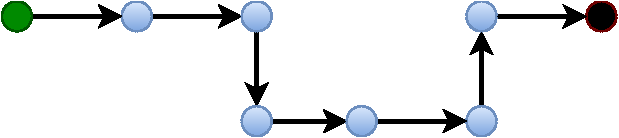
\includegraphics[width=.6\textwidth]{grafim.pdf}
  \end{figure}
\end{frame}
}

% Porém essa representação começa a apresentar problemas quando o número
% de elementos aumenta (cruzamentos, sobreposição) como na figura do tráfego aéreo, fica difícil enxergar
% as conexões entre aeroportos, etc
\setbeamercolor{background canvas}{bg=white}
\begin{frame}{Visualização de Dados do Tráfego}
  \begin{figure}[!htb]
    \centering
    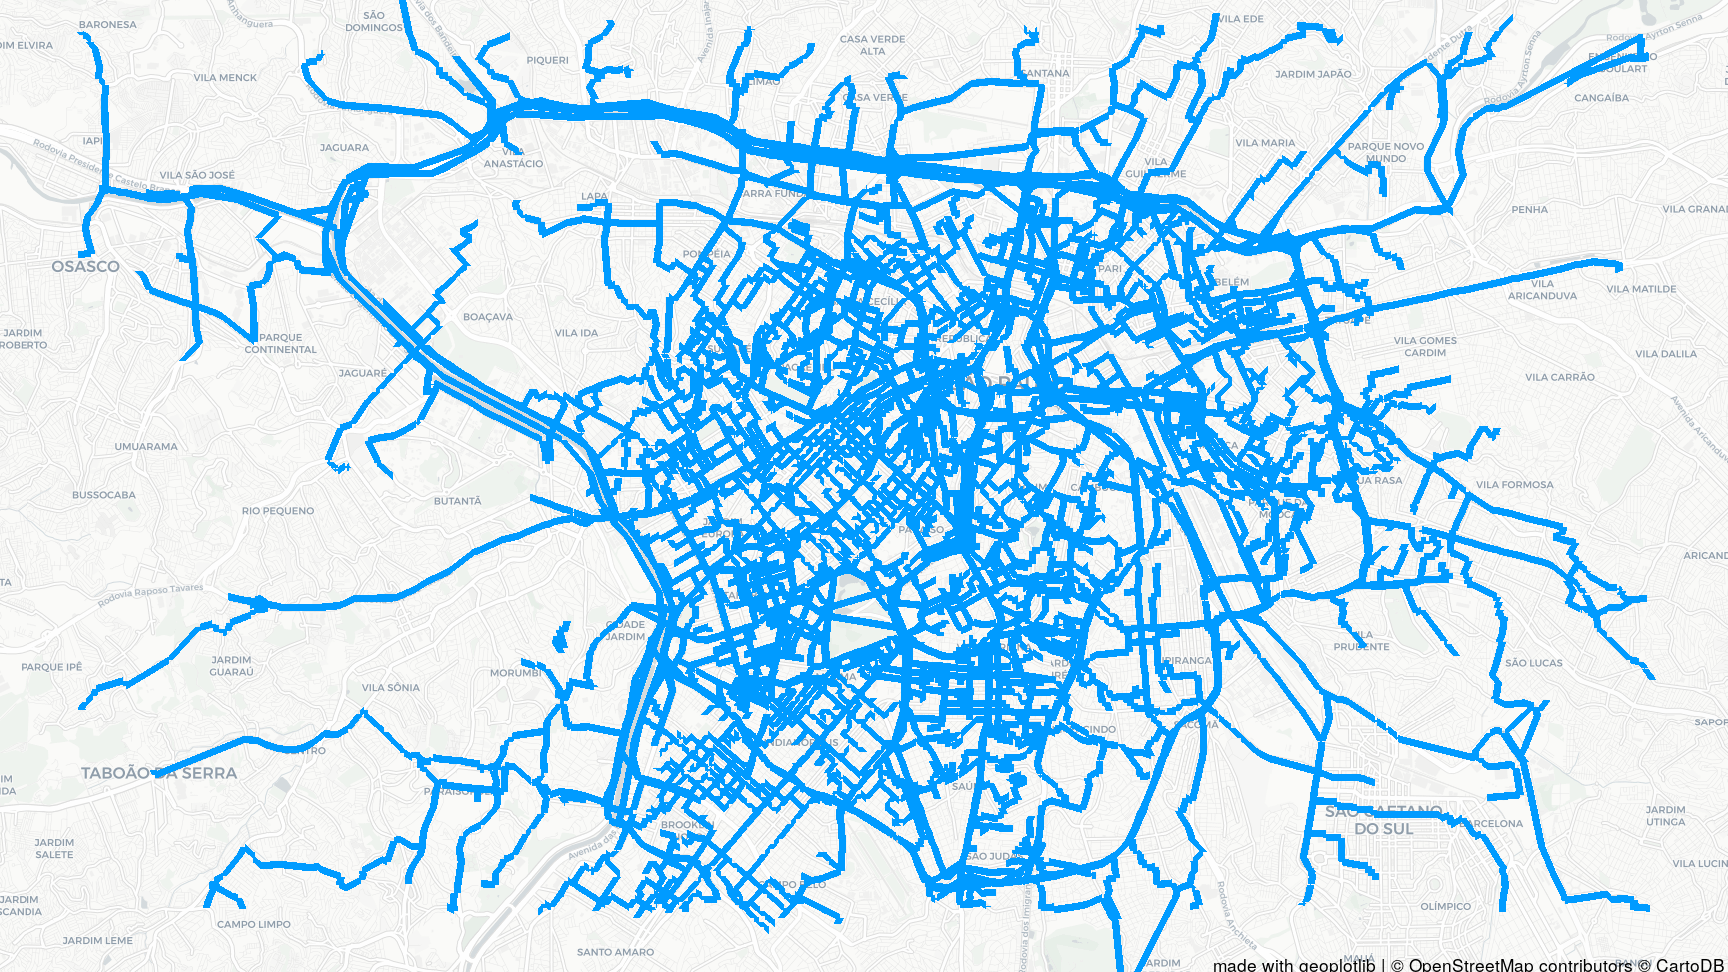
\includegraphics[width=\textwidth]{../figuras/trafego-ocluso.png}
  \end{figure}
\end{frame}

% Aqui eu introduzo o bundling como solução para simplificar a visualização
% desse tipo de representação agrupando-se as arestas similares por algum
% critério

% No caso do transito esse critério tem q levar em conta a
% direção dos fluxos

% Com ela podemos ver A ESTRUTURA GERAL dos dados.

% Citar ainda que existem maneiras diferentes de se atingir um "bundling"
{
\setbeamercolor{background canvas}{bg=white}
\begin{frame}{Bundling}
  \begin{figure}[!htb]
    \centering
    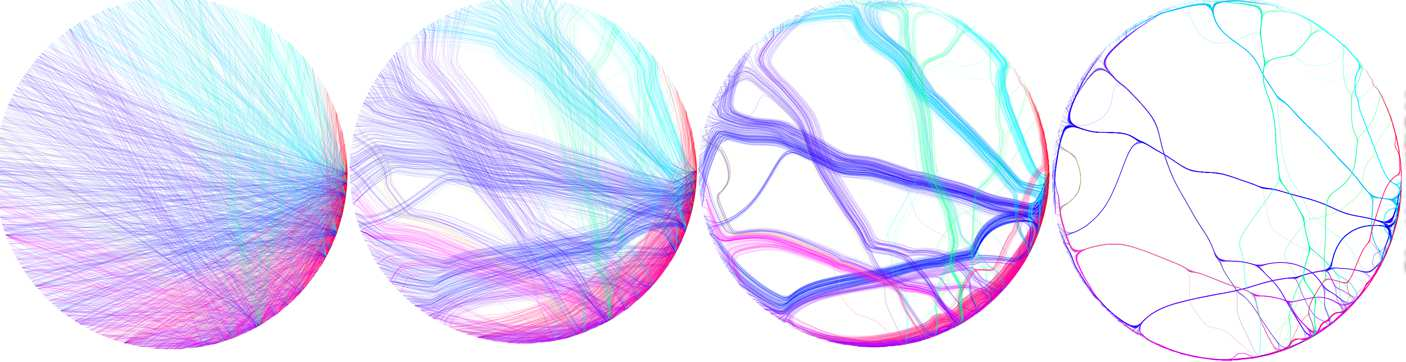
\includegraphics[width=1\textwidth]{bundle-ex.png}
  \end{figure}

  \pause
  \begin{itemize}
    \item Reduz a oclusão agrupando arestas similares
    \item Cria uma nova abstração da estrutura geral dos dados
  \end{itemize}
\end{frame}
}

% Existem algumas aplicações para visualização de trânsito bem conhecidas
% Mas elas focam em visualizações pontuais do trânsito e não na sua estrutura geral
% Outra coisa, por exemplo, não é possível saber as origens que geram um
% determinado engarrafamento em uma via
\begin{frame}{Aplicações de Visualização do Trânsito}
  \centering
  Google Maps - Waze - OlhoVivo
  \begin{figure}[!htb]
    \centering
    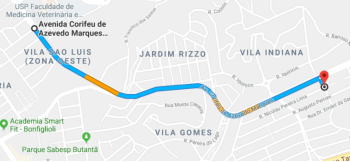
\includegraphics[width=\textwidth]{maps.pdf}
  \end{figure}
 \end{frame}

% Aqui eu falo as explicações dadas no texto para cada pergunta
\begin{frame}{Questões de Pesquisa}
  \begin{block}{Explorar a técnica de \emph{bundling} na visualização dos fluxos de origem e destino}
    \begin{enumerate}
      \pause
      \item Como o bundling pode ser usado para identificar os fluxos de origem
      e destino no trânsito em diferentes escalas?

      \pause
      \item É possível utilizar o bundling para identificar padrões de fluxos
      de origem e destino no trânsito?

      \pause
      \item O bundling é eficiente para gerar uma visualização de uma grande
      quantidade de dados do trânsito?
    \end{enumerate}
  \end{block}
\end{frame}

% A ideia é mostrar que não é só aplicar bundling nos dados e ver no que dá
%\begin{frame}{Desafios}
%    \begin{itemize}
%      \item Selecionar um método de bundling
%
%      \item Elaborar cenários e obter dados para validar nossa abordagem
%
%      \item Implementar e testar visualização
%    \end{itemize}
%\end{frame}

% Necessário explicar mais afundo o modelo de bundling, principalmente
% nas questões dos atributos de densidade e direção que queremos destacar
% para visualizar os fluxos de origem e destino
\section{Conceitos}

\begin{frame}{Métodos de \emph{bundling}}
  \begin{figure}[!htb]
    \centering
    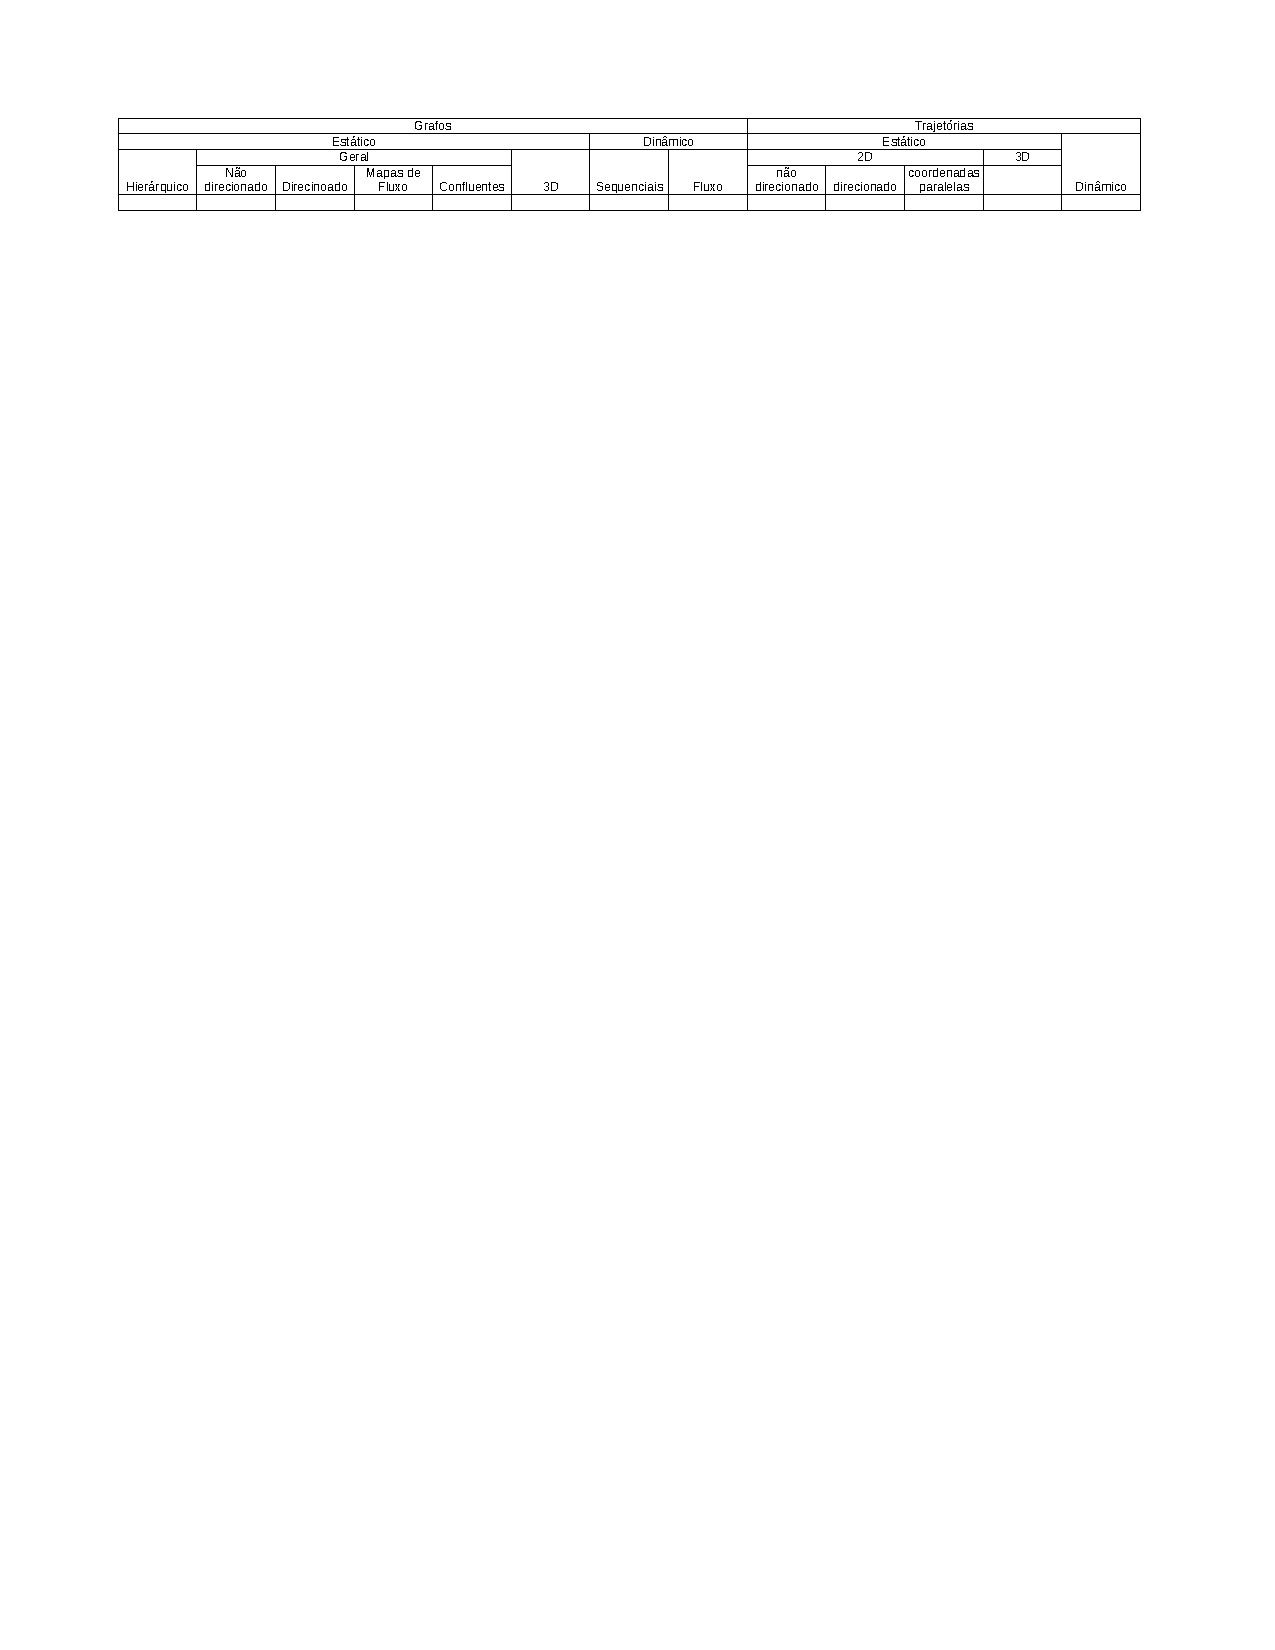
\includegraphics[width=\textwidth]{estado-da-arte.pdf}
  \end{figure}

\hfill \citep{Lhuillier2017}
\end{frame}

\begin{frame}{\emph{Attribute-Driven Edge Bundling} - ADEB}
  \begin{itemize}
    \item Algoritmo rápido e eficiente (paralelizável na GPU)
    \item Consegue utilizar atributos no critério de similaridade (direção)
  \end{itemize}
\end{frame}

\begin{frame}{\emph{Attribute-Driven Edge Bundling} - ADEB}
  \begin{enumerate}
    \item Converter o grafo G em um mapa de densidade usando uma função de densidade
    \item Computar o gradiente da função de densidade para cada ponto/nó do grafo
    \item Mover os nós na direção do gradiente (áreas mais densas)
  \end{enumerate}
\end{frame}

\section{Trabalhos Relacionados}

% Analisando alguns trabalhos relacionados sobre visualização
\begin{frame}{Trabalhos relacionados}
  \begin{itemize}
    \item Tipo de dado

    \item Propriedades espaciais e temporais

    \item Agrupamento (regiões, dias de semana)
  \end{itemize}
\end{frame}

\begin{frame}{Trabalhos relacionados}
\begin{figure}[ht!]
  \centering
  \begin{subfigure}[t]{0.45\textwidth}
    \centering
    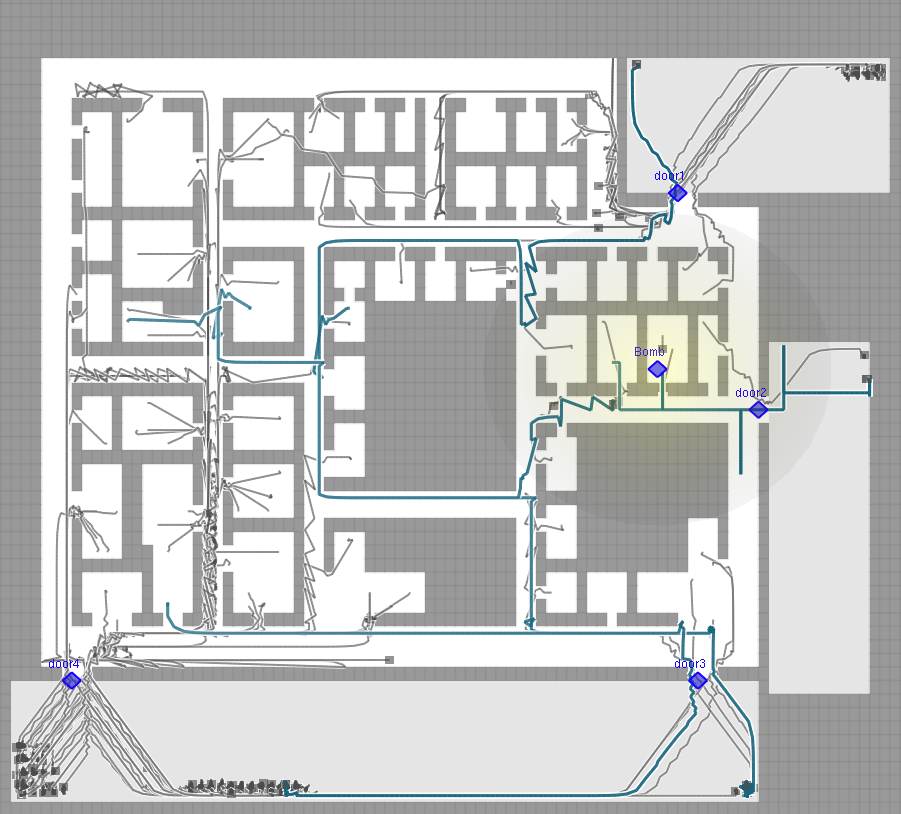
\includegraphics[width=\textwidth]{../figuras/proximidade-espacial.png}
  \end{subfigure}
  ~
  \begin{subfigure}[t]{0.45\textwidth}
    \centering
    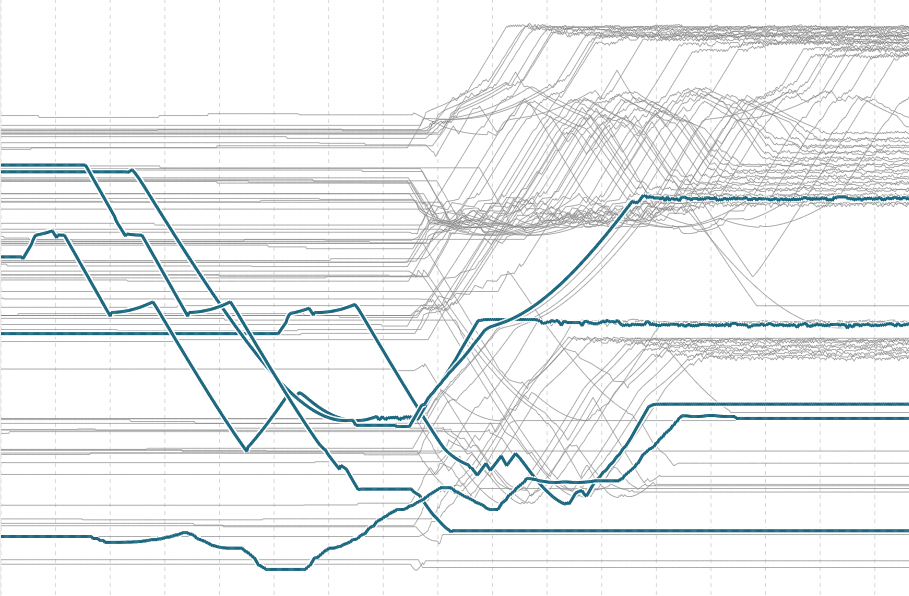
\includegraphics[width=\textwidth]{../figuras/proximidade-abstrata.png}
  \end{subfigure}
\end{figure}
  \centering
  Leiaute espacial \emph{vs.} abstrato
\end{frame}

\begin{frame}{Trabalhos relacionados}
  \begin{figure}[!h]
    \centering
    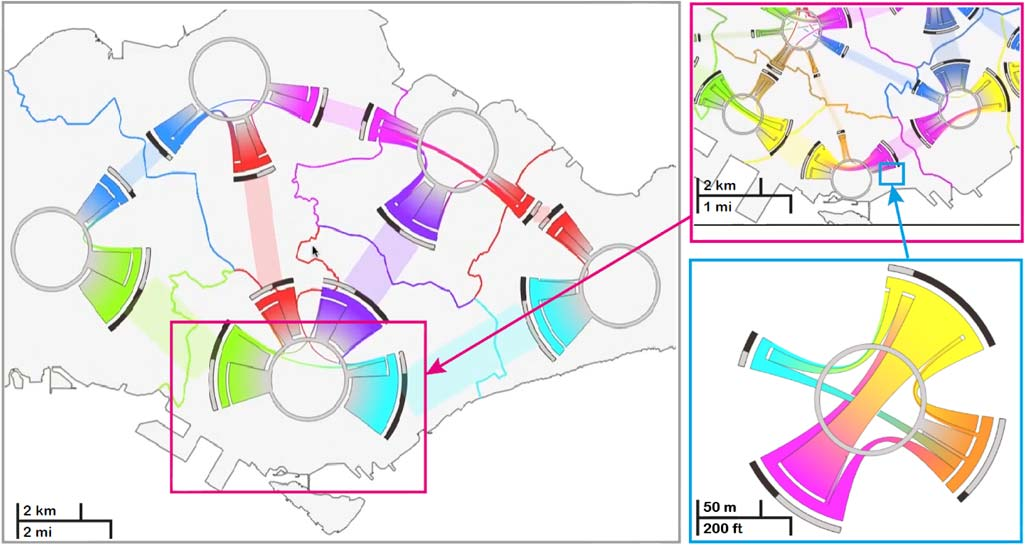
\includegraphics[width=0.97\textwidth]{../figuras/region-based.png}
  \end{figure}
\end{frame}

\begin{frame}{Trabalhos relacionados}
  \begin{tabular}{|c|c|c|c|}
    \hline
    \textbf{Trabalho}       & \textbf{Dados do Trânsito} & \textbf{\emph{Bundling}} & \textbf{Leiaute}  \\ \hline
    Nossa proposta          & \checkmark                 & \checkmark               &          linhas   \\ \hline
    \citet{Kim2018}         & x                          &  x                       &          linhas   \\ \hline
    \citet{Andrienko2017}   & \checkmark                 &  x                       &          radial   \\ \hline
    \citet{Anita2017}       & x                          & \checkmark               &          linhas   \\ \hline
    \citet{Landersberg2016} & x                          &  x                       &          linhas   \\ \hline
    \citet{Klein2014}       & x                          & \checkmark               &          linhas   \\ \hline
    \citet{Chu2014}         & x                          &  x                       &          variado  \\ \hline
    \citet{Ferreira2013}    & \checkmark                 &  x                       &          pontos   \\ \hline
    \citet{Zeng2013}        & x                          & \checkmark               &          radial   \\ \hline
    \citet{Guo2011}         & \checkmark                 &  x                       &          variado  \\ \hline
  \end{tabular}
\end{frame}

\section{Metodologia}

\begin{frame}{Implementação}
  \begin{itemize}
    \item Poucos algoritmos de bundling estão disponíveis em bibliotecas
    \item A maioria dos trabalhos não disponibilizam o código fonte
  \end{itemize}
\end{frame}

% Uma ferramenta que faz parte do ecossistema InterSCity, feita para integrar
% com o InterSCImulator, a qual estamos desenvolvendo para validarmos nossa abordagem
{
\setbeamercolor{background canvas}{bg=white}
\begin{frame}{InterSCityPlotter}
  \begin{figure}[!htb]
    \centering
    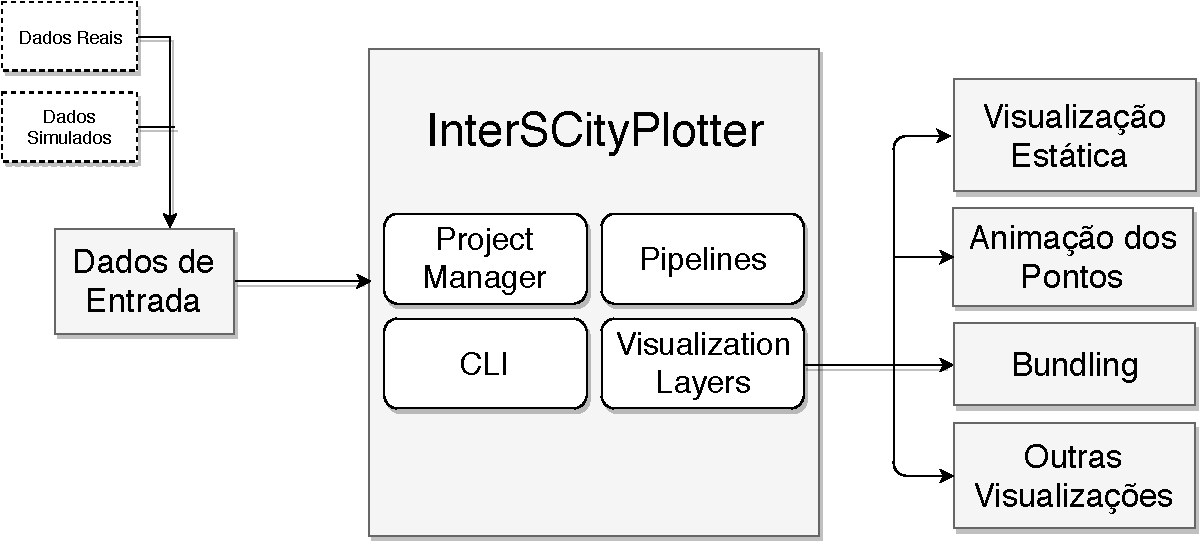
\includegraphics[width=1\textwidth]{interscityplotter.pdf}
  \end{figure}
\end{frame}
}

% Utilizaremos dois conjuntos de dados em nossa análise
% Os dados possuem o registro da posição e do tempo ao longo de toda a trajetória
% desde a origem até o destino

% as questões de pesquisa, principalmente Q2 e Q3 no caso dos dados simulados
\begin{frame}{Conjuntos de Dados}
  \begin{itemize}
    \item Tráfego simulado (carros e ônibus)
    \item Tráfego de ônibus na cidade de SP
  \end{itemize}

  \begin{center}
  $T = \left\langle p_i = ((latitude, longitude) \in \mathbb{R}^2, t \in \mathbb{R}^+, a^n \in \mathbb{R})_i \right\rangle$
  \end{center}
\end{frame}

% Os dados precisarão ainda passar por algumas etapas de limpeza
% eventualmente precisamos checar possíveis inconsistências ou ruídos
\begin{frame}{Conjuntos de Dados (pré-processamentos)}
  \begin{itemize}
    \item Viagens da simulação não finalizadas
    \item Dados inconsistentes com a trajetória
    \item Rotas circulares
    \item Anomalias
    \item Derivação da direção
  \end{itemize}
\end{frame}

% Então chega a parte importante, que é a nossa proposta para visualização
% dos fluxos de OD com bundling. Geralmente sempre vai ter um tradeoff de informações
% em cada escolha feita. 
\begin{frame}[standout]
  Proposta de Visualização: codificar visualmente as propriedades espaciais
e temporais dos dados.
\end{frame}

% Para visualizar os fluxos de OD no trânsito, estamos interessados na sua direção
% e na sua densidade
\begin{frame}{Visualização dos fluxos de OD}
  \begin{itemize}
    \item Direção
    \item Densidade
    \item Padrões de deslocamento em um dado momento
    \item Mudanças ao longo do tempo
  \end{itemize}
\end{frame}

% A primeira decisão que tomamos foi projetar os dados sobre um mapa,
% pois ele traz um foco que mostra intuitivamente as propriedades espaciais
% que ajuda a manter um mapa mental de localidade entre as regiões
\begin{frame}{Leiaute da Visualização}
  \begin{columns}[t]
    \col
		\begin{figure}[ht!]
			\centering
			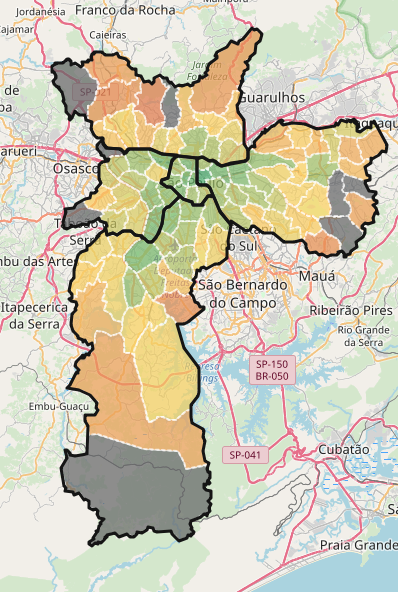
\includegraphics[width=.65\textwidth]{sp-map.png}
		\end{figure}

    \col
		\begin{coloredblock}{white!90!white}{}
		Uma projeção sobre um mapa mostra intuitivamente as relações de localidade entre
		as regiões

    \pause
    Para explorar as propriedades temporais  utilizamos um filtro para selecionar
    janelas de tempo em um intervalo $\Delta~t$ 
		\end{coloredblock}
  \end{columns}
\end{frame}

% A agregação com bundling vai dar a estrutura geral do tráfego que estamos
% interessados, destacando os padrões de comportamento em um dado instante do tempo
% Combinado com o parÂmetro temporal, pretendemos visualizar essa estrutura
% em vários momentos do dia, como em horários de pico

% porém, perdemos a capacidade de visualizar viagens individuais, já que
% estamos provendo uma visualização agregada dos dados
\begin{frame}{Agregação Espacial com Bundling}
  \begin{itemize}
    \item Agrupamento das trajetórias com origem-destino e direção similares
    \item Destaque da estrutura geral dos fluxos e seu comportamento
  \end{itemize}
\end{frame}


\begin{frame}{Agregação Espacial Multiescala}
	\begin{figure}[!htb]
		\centering
		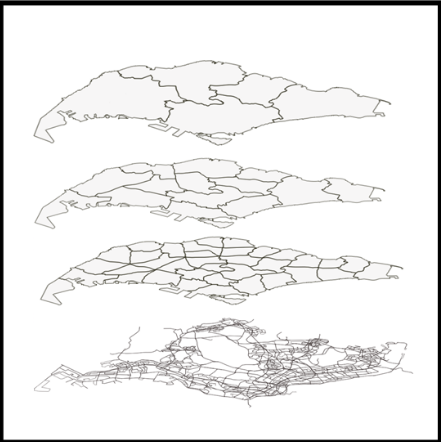
\includegraphics[width=55mm]{multi-scale.png}
	\end{figure}
	\centering
  Quanto menor a escala, mais detalhes sobre o fluxo são obtidos
\end{frame}

% A dimensão espacial é o nosso segundo parâmetro multiescala dentro da visualização
% Queremos explorar os fluxos em diferentes níveis de detalhe com bundling
% pra isso determinamos o conceito de sub-trajetórias, 
% Permite a navegação na dimensão espacial dos dados
\begin{frame}{Agregação Espacial Multiescala}
  \begin{itemize}
    \item Detectamos as sub trajetórias na nova escala
    \item Em seguida reaplicamos bundling no subconjunto
  \end{itemize}
\end{frame}

\begin{frame}{Visualização da Atributos}
	\begin{figure}[ht!]
		\centering
		\begin{subfigure}[t]{\textwidth}
			\centering
			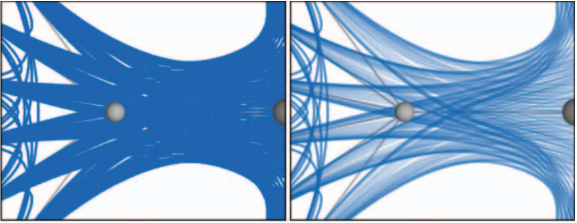
\includegraphics[width=.6\textwidth]{alpha-blending.pdf}
		\end{subfigure}
		~
		\begin{subfigure}[t]{\textwidth}
			\centering
			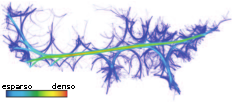
\includegraphics[width=.6\textwidth]{color-density.pdf}
		\end{subfigure}
	\end{figure}
\end{frame}

\begin{frame}{Visualização dos Atributos}
	\begin{figure}[ht!]
		\centering
		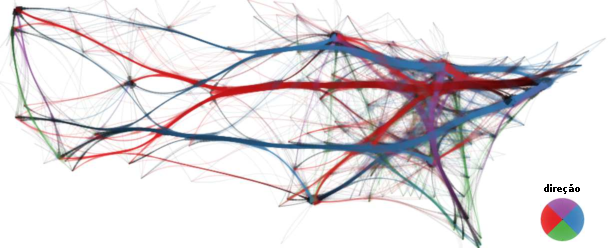
\includegraphics[width=.8\textwidth]{color-wheel.pdf}
	\end{figure}
\end{frame}

% Avaliar uma visualização é uma tarefa complexa e não existem métodos
% objetivos bem estabelecidos na comunidade de visualização. Avaliaremos
% nossa proposta em aspectos qualitativos e quantitativos
\begin{frame}{Validação}
	\centering
 ``Ainda não se tem um consenso sobre métodos para avaliar a
qualidade de uma visualização, ou mesmo critérios objetivos para definir o
que é um bom \emph{bundling}''

	\hfill \citep{Lhuillier2017}.
\end{frame}

\begin{frame}{Validação}
	\textbf{Q1 - Bundling Multiescala:} uma observação objetiva sobre os
diferentes resultados gerados com a variação dos parâmetros de escala espacial
e também temporais, além da forma como apresentamos os atributos de densidade e
direção dos fluxos.
\end{frame}

\begin{frame}{Validação}
	\textbf{Q2 - Padrões ao longo do tempo e na ocorrência de eventos atípicos:} uma observação objetiva dos
resultados gerados pelo experimento onde propomos o bloqueio controlado de vias
da cidade para identificar os impactos no trânsito sobre a ótica da nossa
visualização.
\end{frame}

\begin{frame}{Validação}
	\textbf{Q3 - Eficiência computacional da visualização:} uma medida
quantitativa do tempo de processamento para gerar a visualização de uma grande
quantidade de dados do trânsito gerados com o InterSCSimulator, em um cenário
com 31 milhões de pontos e mais de 585 mil viagens.	
\end{frame}

\section{Considerações Finais}

\begin{frame}{Considerações Finais}
	Esforço Técnico:
	\begin{itemize}
		\item Implementada a arquitetura básica do InterSCityPlotter
		\item Parte dos dados da simulação do tráfego já adquiridos
		\item Os dados dos ônibus ainda serão coletados
	\end{itemize}

	%Validação:
	%\begin{itemize}
	%	\item Avaliamos uma comparação com a visualização de \citet{Guo2011}
	%\end{itemize}
\end{frame}

\begin{frame}{Plano de Trabalho}
\begin{figure}[!htb]
  \centering

  \begin{ganttchart}{2019-02}{2019-11}
    \gantttitlecalendar{year,month=shortname} \ganttnewline

    \ganttbar[progress=15]{Desenvolvimento da visualização}{2019-3}{2019-5} \ganttnewline
    \ganttbar[progress=15]{Coleta e tratamento dos dados}{2019-3}{2019-4}\ganttnewline
    \ganttbar[progress=0]{Execução dos experimentos}{2019-6}{2019-7} \ganttnewline
    \ganttbar[progress=0]{Análise dos resultados}{2019-8}{2019-8} \ganttnewline
    \ganttbar[progress=0]{Escrita da Dissertação}{2019-8}{2019-10} \ganttnewline
    \ganttbar[progress=0]{Escrita de Artigo}{2019-9}{2019-10} \ganttnewline
    \ganttmilestone{Defesa}{2019-10}
  \end{ganttchart}

  \caption{Cronograma.\label{fig:gantt}}
\end{figure}

\end{frame}

\section{Referências}

\begin{frame}[allowframebreaks]{Referências}
  \nocite{bronevetsky02, schmidt03:MSc, FSF:GNU-GPL, CORBA:spec, MenaChalco08, natbib, biblatex, eco:09}
  \printbibliography
\end{frame}

% Recapitulando
\begin{frame}{\insertshorttitle}
  \overview

  % \begin{center} acrescenta espaço vertical;
  % como possivelmente temos bem pouco espaço aqui,
  % vamos usar centering
  {%
    \centering\noindent%
    \url{https://github.com/tallysmartins/interscity-plotter}\par
  }

\end{frame}

\showqrcode

\appendix

%\begin{frame}{Extra info}
%  \begin{itemize}
%    \item It is often useful to have some extra slides addressing likely questions from the audience at the end of the presentation
%    \item By putting them after the ``appendix'' command, they are not counted in the page count indicator
%  \end{itemize}
%\end{frame}
